%
%Let $\mr \in \mrspace$ be a \meaningrepresentation~with a \dialogueact~$\mrtok_0$
%and $\mrSize$ \attributevalues~$\mrtok_1,\ldots,\mrtok_\mrSize$, and let
%$\utttoks = \left[\utttok_1,\ldots,\utttok_\uttSize\right]$ be 
%an utterance that denotes $\mr$, which we write as $\denotes{\utttoks} = \mr$.
%A contiguous span of utterance tokens $\utttoks_{i:j} = \left[\utttok_i,\ldots,\utttok_j\right]$, for $i \le j$, 
%can denote zero or more \attributevalues, that is,
%$\denotes{\utttoks_{i:j}} = \{\mrtok_{k_1}, \mrtok_{k_2}, \ldots\}$. We further define a ``denotation
%set'' of $\mr$ and $\utttoks$ as $\denotationset = \left\{(i^{(k)},j^{(k)}): k \in \left\{1,\ldots,\mrSize\right\} \right\}$ where 
%$\denotes{\utttoks_{i^{(k)}:j^{(k)}}} = \{ \mrtok_k \}$. In other words,
%$\denotationset$ is the set of utterance token spans that denote a single
%\attributevalue.
%
%\autoref{fig:explans} shows an example of controllable \surfacerealization~for the \meaningrepresentation
% \begingroup
% \renewcommand*\arraystretch{.6}
%\begin{align} \mr =  \left[\!\!\left[ \begin{array}{l} (\mrtok_0)\; \textsc{Inform} \\ (\mrtok_1)\; \textrm{name=Aromi} \\ (\mrtok_2)\; \textrm{area=city centre} \\ (\mrtok_3)\; \textrm{eat\_type=coffee shop} \end{array} \right]\!\!\right]\label{eqn:mr1}\end{align}
%\endgroup
%when following either one of two different linearizations \[\ls^{(1)}(\mr) = \left[ \mrtok_0, \mrtok_1, \mrtok_3, \mrtok_2 \right]\quad \textrm{and} \quad \ls^{(2)}(\mr) = \left[ \mrtok_0, \mrtok_3, \mrtok_2, \mrtok_1 \right].\] When using a controllable model, 
%we refer to a linearization $\ls$ as an \utteranceplan. In this work, 
%a \linearizationstrategy~will only permute the location of \attributevalue~tokens, while the \dialogueact~token $\mrtok_0$ will always occupy the first
%position of any \meaningrepresentation~token sequence $\mrtoks$. 
%
%
%
%\begin{figure}
%\begin{subfigure}{\textwidth}
%\caption{~~~~~~~~~~~~~~~~~~~~~~~~~~~~~~~~~~~~~~~~~~~~~~~~~~~~~~~~~~~~~~~~~~~~~~~~~~~~~~~~~~~~~~~~~~~~~~~~~~~~~~~~~~~~~~~~~~~~~~~~~~~~~~~~~~~~~~~~~~~~~~~~~~~~~~~~~~~~~~~~~~~~~~~~~}
%\center
%\fbox{\begin{minipage}{0.87\textwidth}
%\begin{tabular}{cccccc}
%\multirow{2}{*}{$\ls^{(1)}(\mr) = \Bigg[$} & $x_0$ &   $x_{\pi_1}$ & $x_{\pi_2}$ & $x_{\pi_3}$ & \multirow{2}{*}{$\Bigg]$}\\
%& inform & name=Aromi & eat\_type=coffee shop & area=city center \\
%\end{tabular}
%
%~\\[5pt]
%
%\begin{tabular}{cccccccccccc}
%\multirow{2}{*}{~~~~~~$\utttoks^{(1)} = \Bigg[$} & $y_1$ & $y_2$ & $y_3$ & $y_4$ & $y_5$ & $y_6$ & $y_7$ & $y_8$ & $y_9$ & $y_{10}$ & \multirow{2}{*}{$\Bigg]$} \\
%&Aromi & is & a & coffee & shop & in & the & city & centre & . \\
%\end{tabular}
%
%~\\[5pt]
%
%\begin{tabular}{ccccc}
% \multirow{2}{*}{~~$\denotationset_{\mr,\utttoks^{(1)}} = \Bigg\{$} & $(i^{(\pi_1)},j^{(\pi_1)})$ & 
%    $(i^{(\pi_2)},j^{(\pi_2)})$ & 
%    $(i^{(\pi_3)},j^{(\pi_3)})$ & \multirow{2}{*}{$\Bigg\}$}  \\
%   &  (1, 1) & (2, 5) & (6, 9) 
%\end{tabular}
%
%
%\begin{center}
%\begin{tabular}{ccc}
%$\utttoks^{(1)}_{i^{(\pi_1)}:j^{(\pi_1)}}$ & 
%$\utttoks^{(1)}_{i^{(\pi_2)}:j^{(\pi_2)}}$ &
%$\utttoks^{(1)}_{i^{(\pi_3)}:j^{(\pi_3)}}$   \\
%\cmidrule(lr){1-1}
%\cmidrule(lr){2-2}
%\cmidrule(lr){3-3}
%    $\left[\textrm{Aromi}\right]$ & $\left[\textrm{is a coffee shop}\right]$ &
%        $\left[\textrm{in the city center}\right]$ \\ 
%\end{tabular}
%\end{center}
%\end{minipage}}
%\end{subfigure}
%
%%Aromi\textsubscript{1} is\textsubscript{2} a\textsubscript{3} coffee\textsubscript{4} shop\textsubscript{5} in\textsubscript{6} the\textsubscript{7} city\textsubscript{8} centre\textsubscript{9} .\textsubscript{10}
%
%~\\
%~\\
%
%\begin{subfigure}{\textwidth}
%\caption{~~~~~~~~~~~~~~~~~~~~~~~~~~~~~~~~~~~~~~~~~~~~~~~~~~~~~~~~~~~~~~~~~~~~~~~~~~~~~~~~~~~~~~~~~~~~~~~~~~~~~~~~~~~~~~~~~~~~~~~~~~~~~~~~~~~~~~~~~~~~~~~~~~~~~~~~~~~~~~~~~~~~~~~~~}
%\begin{tabular}{cccccc}
%\multirow{2}{*}{$\ls^{(2)}(\mr) = \Bigg[$} & $x_0$ &   $x_{\pi_1}$ & $x_{\pi_2}$ & $x_{\pi_3}$ & \multirow{2}{*}{$\Bigg]$}\\
%& inform & eat\_type=coffee shop & area=city center & name=Aromi\\
%\end{tabular}
%
%~\\[5pt]
%
%\begin{tabular}{cccccccccccccc}
%\multirow{2}{*}{~~~~~~$\utttoks^{(2)} = \Bigg[$} & $y_1$ & $y_2$ & $y_3$ & $y_4$ & $y_5$ & $y_6$ & $y_7$ & $y_8$ & $y_9$ & $y_{10}$ & $y_{11}$& $y_{12}$ & \multirow{2}{*}{$\Bigg]$} \\
%&For & coffee & in & the & centre & of & the & city & , & try & Aromi & .\\
%\end{tabular}
%
%~\\[5pt]
%
%\begin{tabular}{ccccc}
% \multirow{2}{*}{~~$\denotationset_{\mr,\utttoks^{(2)}} = \Bigg\{$} & $(i^{(\pi_1)},j^{(\pi_1)})$ & 
%    $(i^{(\pi_2)},j^{(\pi_2)})$ & 
%    $(i^{(\pi_3)},j^{(\pi_3)})$ & \multirow{2}{*}{$\Bigg\}$}  \\
%   &  (1, 2) & (3, 8) & (11, 11) 
%\end{tabular}
%
%~\\[5pt]
%
%\begin{tabular}{ccc}
%$\utttoks^{(2)}_{i^{(\pi_1)}:j^{(\pi_1)}}$ & 
%$\utttoks^{(2)}_{i^{(\pi_2)}:j^{(\pi_2)}}$ &
%$\utttoks^{(2)}_{i^{(\pi_3)}:j^{(\pi_3)}}$   \\
%    $\left[\textrm{For coffee}\right]$ & $\left[\textrm{in the centre of the city}\right]$ &
%        $\left[\textrm{Aromi}\right]$ \\ 
%\end{tabular}
%\end{subfigure}
%
%~\\
%
%\caption{Examples of two possible utterance plans for $\mr$ (defined \autoref{eqn:mr1}) implied by
%the linearizations $\ls^{(1)}$ (a) and $\ls^{(2)}$ (b), their realizations $\utttoks$, denotation sets $\denotationset_{\mr,\utttoks}$, and corresponding
%attribute-value spans $\utttoks_{i:j}$.}
%\label{fig:explans}
%\end{figure}











%Assume we have a
%training corpus $\corpus = \left\{\left(\mr^{(1)}, \utttoks^{(1)}\right), \ldots, \left( \mr^{(\corpusSize)}, \utttoks^{(\corpusSize)}\right) \right\}$
%
%%That is, given such a model $\model$,
%% a \dialogueact~$\mrtok_0$ a series of \attributevalues~$\mrtok_1,\mrtok_2,\ldots,\mrtok_\mrSize$, the conditional distribution,
%%\[\model\left(\cdot|\mrtok_0,\mrtok_1,\ldots,\mrtok_\mrSize;\params\right)\]
%%prefers utterances $\utttoks$ such that \attributevalues~are realized 
%%in the order specified 
%
%In the \alignmenttraining~linearization,
%during training the order of
%attribute-value pairs $\attr_1, \attr_2, \ldots, \attr_\size{\mr}$
%matches the order in which they are realized in the
%corresponding training utterance.
%This is feasible because in the majority of cases, there is a one-to-one
%mapping of attribute-values and utterance sub-spans.
%
%
%We obtain this ordering using a manually constructed set of matching rules
%to identify which utterance sub-spans correspond to each attribute-value
%pair (see \autoref{sec:align}).

\begin{figure}
    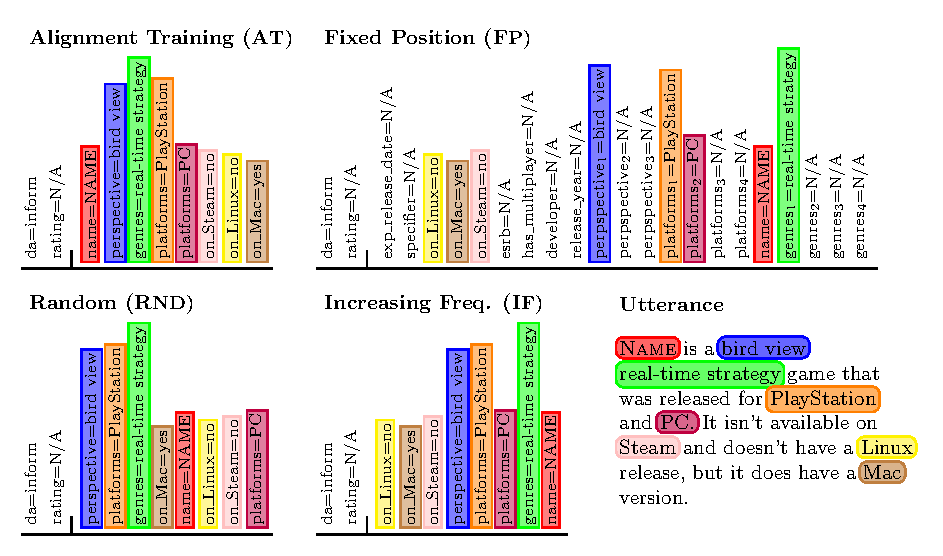
\includegraphics{nlg/inputordering.pdf}
\end{figure}



\newcommand{\lsname}[1]{\textsc{#1}}
\newcommand{\lsshort}[1]{\textsc{#1}}
\newcommand{\acount}{n}
\newcommand{\size}[1]{|#1|}
\newcommand{\lin}{\pi}
\newcommand{\valstr}[1]{\textit{#1}}
\newcommand{\uttstr}[1]{\textit{#1}}
\newcommand{\alignshort}{AT}
\newcommand{\enc}{Enc}
\newcommand{\rep}{h}
\newcommand{\attrval}[2]{#1=#2}
\newcommand{\phraseAug}{+p}
\newcommand{\bleu}{\textsc{Bleu}}
\newcommand{\rougel}{\textsc{Rouge-L}}
\newcommand{\biGRU}{biGRU}
\newcommand{\BgUP}{\textsc{BgUP}}
\newcommand{\NUP}{\textsc{NUP}}
\newcommand{\DA}[1]{\textsc{#1}}
\newcommand{\Oracle}{\textsc{Oracle}}
\newcommand{\BART}{BART}
\newcommand{\Transformer}{Transformer}

\subsubsection{Alternative Linearization Strategies}

\paragraph{Random (\textsc{Rnd})} In the \lsname{random} linearization (\lsshort{Rnd}), we randomly
order the attribute-value pairs for a given MR. This strategy 
serves as a baseline for determining
if linearization ordering matters at all for faithfulness. \lsshort{Rnd} 
is similar to token level noise used in
sequential denoising autoencoders \cite{wang2019denoising} and might even improve faithfulness.
During training, we resample the ordering for each example at every epoch.
We do not resample the validation set in order to obtain stable results 
from which to pick the best model.

\paragraph{Increasing Frequency (\textsc{If})} 
In the \lsname{increasing frequency} linearization (\lsshort{If}), 
we order the attribute-value pairs by increasing frequency of 
occurrence in the training data
i.e. $\acount(\attr_i) \le \acount(\attr_{i+1})$.
We hypothesize that placing frequently occurring items in a consistent location
may make it easier for $\model$ to realize those items correctly, possibly
at the expense of rarer items.

\paragraph{Fixed Position (\textsc{Fp})} We take  consistency one step further 
and create a fixed ordering of all attributes, \textit{n.b.} not attribute-values, ordering them in increasing
frequency of occurrence on the training set (i.e. every instance has the same
order of attributes in the encoder input). In this \lsname{fixed position}
linearization (\lsshort{Fp}), attributes that are not present 
in an MR are explicitly represented with an \valstr{N/A} value. 
For list-valued slots, we determine the maximum length list in the training
data and create that many repeated slots in the input sequence.
This linearization is feasible for datasets with a modest number of 
unique attributes (in our case Viggo has 14 attributes and
E2E eight) but would not easily scale to 10s, 100s, or larger
attribute vocabularies. 




Crucially, \alignmenttraining~stands in contrast to the  first three strategies
(\lsshort{Rnd}, \lsshort{If}, and \lsshort{Fp}) which do not have any
correspondence between the the order of attribute-value pairs in $\lin(\mr)$
and the order in which they are realized in the corresponding
utterance $\utttoks$.


%At test time, when there is no reference utterance \lsshort{At}
%cannot specify a linearization. However, models trained with \lsshort{At}
%can generate an  utterance from an arbitrary utterance plan
%$\attr_1, \attr_2, \ldots, \attr_{\size{\mr}}$
%provided by an external source, such as an utterance planner model or human
%reference.








\subsection{Models}
\subsubsection{Generation Models}
We examine the effects of linearization strategy and data augmentation
on a bidirectional gated recurrent units with attention (biGRU)
and Transformer based S2S models.
Hyper-parameters were found using grid-search, selecting the model
with best validation \textsc{Bleu} \cite{papineni2002bleu} score. We performed a separate
grid-search for each architecture-linearization strategy pairing in case
there was no one best hyper-parameter setting.

Additionally, we
fine-tune BART \cite{lewis2019bart}, a large pretrained Transformer-based S2S model. We stop fine-tuning after validation set cross-entropy stops decreasing.
%lowest validation set cross-entropy. 

\paragraph{biGRU Model}
Let $\mathcal{V}$ be the encoder input vocabulary, and  $V \in\mathbb{R}^{\size{\mathcal{V}}\times 512}$ its associated embedding matrix, and let
$V_v \in \mathbb{R}^{512}$ be the associated embedding for
each $v \in \mathcal{V}$.

Let the encoder input $\lin(\mr) = v_1, v_2, \ldots, v_{\size{\mr}}$.
The hidden states of the first GRU encoder layer are computed as
\begin{align*}
        \overrightarrow{h}_0 & =\overleftarrow{h}_{\size{x} + 1}  = 0 \\
        \overrightarrow{h}_i &= \overrightarrow{\operatorname{GRU}}(V_{v_i}, \overrightarrow{h}_{i-1}) &
        \textrm{for $i \in 1,\ldots,\size{\mr}$}\\
            \overleftarrow{h}_i &= \overleftarrow{\operatorname{GRU}}(V_{v_i}, \overleftarrow{h}_{i+1}) &
            \textrm{for $i \in 1,\ldots,\size{\mr}$}\\
                h_i^{(1)} & = \left[\overrightarrow{h}_i, \overleftarrow{h}_i\right]
        \end{align*} When using a two layer GRU, we similarly compute
        \begin{align*}
                \overrightarrow{h}^{(2)}_0 & =\overleftarrow{h}^{(2)}_{\size{x} + 1}  = 0 \\
                \overrightarrow{h}^{(2)}_i &= \overrightarrow{\operatorname{GRU}}(h^{(1)}_i, \overrightarrow{h}^{(2)}_{i-1}) &
                \textrm{for $i \in 1,\ldots,\size{\mr}$}\\
                    \overleftarrow{h}^{(2)}_i &= \overleftarrow{\operatorname{GRU}}(h^{(1)}_i, \overleftarrow{h}^{(2)}_{i+1}) &
                    \textrm{for $i \in 1,\ldots,\size{\mr}$}\\
                        h_i^{(2)} & = \left[\overrightarrow{h}^{(2)}_i, \overleftarrow{h}^{(2)}_i\right]
                \end{align*}
                Going forward, let $h_i$ correspond to the final encoder, i.e. $h_i = h_i^{(1)}$
                in the one-layer biGRU case, and $h_i=h_i^{(2)}$ in the two layer case.
                Let $\mathcal{W}$ be the vocabulary of utterance tokens, and $W\in\mathbb{R}^{
                \mathcal{W} \times 512}$ it's associated embedding matrix, and let
                $W_w \in \mathbb{R}^{512}$ be the associated embedding for
                each $w \in \mathcal{W}$.

                Given the decoder input sequence $y = w_1, w_2, \ldots, w_{\size{y}}$,
                we compute the hidden states of the decoder as,
                \begin{align*}
                        g_0 & = \tanh(U^Th_{\size{x}} + u) \\
                        g_i & = \operatorname{GRU}(W_{w_i}, g_{i-1}) & \textrm{for $i \in 1,\ldots, \size{y}$}\\
                        \bar{h}_i & = \sum^{\size{x}}_{j=1}\alpha_{i,j}h_j & \textrm{for $i \in 1,\ldots, \size{y}$}
                \end{align*}
                where $U \in \mathbb{R}^{1024 \times 512}$ and $u \in \mathbb{R}^{512}$
                and $\alpha_{i,j} \in (0, 1), \sum^{\size{x}}_{j=1}\alpha_{i,j} = 1$ is the attention weight of decoder state $i$ on encoder state $j$. We compute
                attention in one of two ways (the attention method is a hyper-paremeter
                option):
                \begin{enumerate}
                    \item Feed-forward ``Bahdanau'' style attention \cite{cho2014learning},
                            also known as ``concat'' \cite{luong2015effective}:
                        \[ \alpha_{i,j} = k^T\tanh\left(K^T \left[\begin{array}{c} g_i \\ h_j\end{array}\right] \right)  \] with $K\in \mathbb{R}^{1536 \times 512}$ and $k \in \mathbb{R}^{512}$.
                        \item ``general'' \cite{luong2015effective} :
                                \[ \alpha_{i,j} = g_i^T K  h_j  \] with $K \in \mathbb{R}^{512 \times 1024}$.
                        \end{enumerate}

                        Finally, for $i \in 1, \ldots, \size{y}-1$ we compute
                        \begin{align*}
                        \bar{g}_i & =  \tanh\left(Q^T\left[\begin{array}{l} g_i\\ \bar{h}\end{array}\right] + q\right) \\
                                p\big(w_{i+1}|w_{\le i}, \lin(\mr)\big) & \propto \exp\left(M_{w_{i+1}}^T\hat{g}_i + m_{w_{i+1}}\right)  
                        \end{align*}
                        where $Q \in \mathbb{R}^{1024 \times 512}$, $q\in\mathbb{R}^{512}$,
                        $m \in \mathbb{R}^{\size{\mathcal{W}}}$,
                        and $M \in \mathbb{R}^{\size{\mathcal{W}} \times 512}$ is the output
                            embedding matrix.
                                As a hyper-paramter setting, we consider tieing the decoder
                                    input and output
                                        embedding matrices, i.e. $W = M$.
                                            Dropout of 0.1 is applied to all embedding, GRU outputs, and linear
                                                layer outputs.


\paragraph{Transformer}
We used the Transformer S2S as implemented in
\href{https://pytorch.org/}{PyTorch}.
The input embedding dimension is 512 and inner hidden layer size is 2048.
We used 8 heads in all multi-head attention layers.
We used Sinusoidal position embeddings following those described in
\citet{rush2018annotated}. Additionally, we used Adam with the learning
rate schedule provided in that work (factor=1, warmup=8000).
Dropout was set to 0.1.


\newcommand{\utt}{\ensuremath{\mathbf{y}}}
\newcommand{\uttVocab}{\ensuremath{\mathcal{W}}}
\newcommand{\da}{\ensuremath{a}}
\newcommand{\inseq}{\mathbf{x}}
\newcommand{\Attrs}{\ensuremath{\mathcal{V}}}
\newcommand{\inSize}{m}
\newcommand{\outSize}{n}

\newcommand{\mmhAttn}{\operatorname{maskedMHAttn}}
\newcommand{\mhAttn}{\operatorname{MHAttn}}

\newcommand{\mrEmb}{\mathbf{W}}
\newcommand{\uttEmb}{\mathbf{V}}
\newcommand{\decInput}{\mathbf{G}}
\newcommand{\decInputi}{\mathbf{g}_i}


\newcommand{\tfeA}{\boldsymbol{\check{\encInput}}^{(i)}}
\newcommand{\tfeB}{\boldsymbol{\bar{\encInput}}^{(i)}}
\newcommand{\tfeC}{\boldsymbol{\hat{\encInput}}^{(i)}}
\newcommand{\tfeD}{\boldsymbol{\dot{\encInput}}^{(i)}}
\newcommand{\tfeE}{\boldsymbol{\ddot{\encInput}}^{(i)}}

\newcommand{\tfdA}{\boldsymbol{\check{\decInput}}^{(i)}}
\newcommand{\tfdB}{\boldsymbol{\bar{\decInput}}^{(i)}}
\newcommand{\tfdC}{\boldsymbol{\hat{\decInput}}^{(i)}}
\newcommand{\tfdD}{\boldsymbol{\grave{\decInput}}^{(i)}}
\newcommand{\tfdE}{\boldsymbol{\tilde{\decInput}}^{(i)}}
\newcommand{\tfdF}{\boldsymbol{\acute{\decInput}}^{(i)}}
\newcommand{\tfdG}{\boldsymbol{\dot{\decInput}}^{(i)}}
\newcommand{\tfdH}{\boldsymbol{\ddot{\decInput}}^{(i)}}


%\subsection{Transformer Model Definition}
%
%Each Transformer layer is divided into blocks which each have three
%parts, (i) layer norm, (ii) feed-forward/attention, and  (iii) skip-connection.
%We first define the components used in the transformer blocks before
%describing the overall S2S transformer. 
%Starting with layer norm \cite{ba2016}, let $\encInput \in \reals^{m\times n}$, then we have
%$\layerNorm : \reals^{m \times n} \rightarrow \reals^{m \times n}$,
%\[\layerNorm(\encInput; \lnweightv, \lnbias) = \lnweight \odot (\encInput - \boldsymbol{\mu}) \odot \Lambda + \mathbf{b} \]
%
%where $\lnweightv, \lnbias \in \reals^n$ are learned parameters, $\odot$ is the elementwise product, $\lnweight = \left[\lnweightv,\ldots,\lnweightv\right] \in \reals^{m\times n}$ is a tiling of the parameter vector, $\lnweightv$, $m$ times, and  $\boldsymbol{\mu}, \boldsymbol{\Lambda} \in \reals^{m\times n}$ are
%defined elementwise as
%\[\boldsymbol{\mu}_{i,j} = \frac{1}{n} \sum_{k=1}^n \encInput_{i,k}\]
%and 
%\[\boldsymbol{\Lambda}_{i,j} = \left(
%    \sqrt{ \frac{1}{n-1} \sum_{k=1}^n \left( 
%\encInput_{i,k} - \boldsymbol{\mu}_{i,j} \right)^2  + \epsilon}\right)^{-1}\]
%respectively. The $\epsilon$ term is a small constant for numerical stability,
%set to $10^{-5}$.
%
%The inplace feed-forward layer, $\feedforward$, is a simple single-layer perceptron
%with $\relu$ activation 
%($\relu(\encInput) = \max\left(\zeroEmb, \encInput\right)$) \cite{nair2010}, applied to each row of an $m \times n$ input matrix, i.e. a sequence of $m$ objects
%with $n$ features,\\
%
%
%\noindent $\feedforward\left(\encInput;\weight{i},\weight{j},\bias{i},\bias{j}\right) =$
%\[  \relu\left(\encInput\weight{i} + \bias{i}\right)\weight{j} + \bias{j}     \]
%where $\weight{i} \in \reals^{\embDim \times \hidDim}$, $\bias{i} \in \reals^{\hidDim}$,
%$\weight{j} \in \reals^{\hidDim \times \embDim}$, $\bias{j} \in \reals^{\embDim}$ are learned parameters and 
%matrix-vector additions (i.e. $\mathbf{X} + \mathbf{b}$) are broadcast across
%the matrix rows.
%
%
%The final component to be defined is the multi-head attention, $\MultiAttn$ which is defined
%as\\
%
%\noindent  $\MultiAttn(\Query, \Key; \weight{a_1}, \weight{a_2}) =$
%\[ \left[ \begin{array}{c} 
%            \Attn\left(\Query\weight{a_1}_{1,1}, \Key\weight{a_1}_{2,1}, \Key \weight{a_1}_{3,1} \right),\\
%    \vdots \\
%            \Attn\left(\Query\weight{a_1}_{1,H}, \Key\weight{a_1}_{2,H}, \Key \weight{a_1}_{3,H} \right)
%\end{array} \right] \weight{a_2}
%\]
%
%where $\left[\cdot \right]$ indicates column-wise concatenation,  $\weight{a_1}_{1,*} \in \reals^{\embDim\times \embDim / H}$
%and $\weight{a_2} \in \reals^{\embDim\times \embDim}$ are learned parameters,
%$H$ is the number of attention heads, and  
%$\Attn$ is defined,
%
%\[\Attn\left(\mathbf{Q}, \mathbf{K}, \mathbf{V}\right) = \softmax\left(\frac{\mathbf{Q} \mathbf{K}^T}{\sqrt{\embDim}} \right)\mathbf{V}. \]
%
%Additionally, there is a masked variant of attention, $\MultiAttn_{M}$
%where the attention is computed 
%
%\[\Attn\left(\mathbf{Q}, \mathbf{K}, \mathbf{V}\right) = \softmax\left(\frac{\mathbf{Q} \mathbf{K}^T \odot \Mask }{\sqrt{\embDim}} \right)\mathbf{V} \]
%where $\Mask \in \reals^{\outSize \times \inSize}$ 
%is a lower triangular matrix, i.e. values on or below the diagonal are 1
%and all other values are $-\infty$. 
%
%Given these definitions, we now define the S2S transformer.
%Let $\Attrs$ be the encoder input vocabulary, and  $\encEmbs \in
%\reals^{\size{\Attrs} \times \embDim}$ an associated word embedding matrix
%where $\encEmbs_\attr \in \reals^{\embDim}$ denotes the $\embDim$-dimensional
%embedding for each $\attr \in \Attrs$. 
%Given a linearized MR $\lin(\mr) = \inseq= \left[ \da, \attr_1, \attr_2, \ldots,
%\attr_{\size{\mr}}\right] \in \Attrs^{\inSize}$ where the length
%of the sequence is $\inSize = \size{\mr} + 1$,
%let $\encWordEmb_i = \encEmbs_{\inseq_i}$ for $i \in \{1, \ldots \inSize\}$.
%
%Additionally let $\posEmb \in \reals^{\inSize_{max} \times \embDim}$ be a sinusoidal position embedding matrix
%defined elementwise with 
%\begin{align*}
%    \posEmb_{i,2j} & = \sin\left(\frac{i}{10,000^{ \frac{2j}{\embDim} }}\right) \\
%    \posEmb_{i,2j+1} & = \cos\left(\frac{i}{10,000^{ \frac{2j}{\embDim} }}\right). 
%\end{align*}
%The encoder input sequence $\encInput^{(0)} \in \reals^{\inSize \times \embDim}$ is then defined by
%\[\encInput^{(0)} = \left[\begin{array}{c} 
%            \encWordEmb_1 + \posEmb_1,\\
%            \encWordEmb_2 + \posEmb_2,\\
%            \vdots \\
%        \encWordEmb_\inSize + \posEmb_\inSize
%    \end{array}
%                        \right] \]
%
% A sequence of $l$ transformer encoder layers are then applied to the encoder
% input, i.e. $\encInput^{(i+1)} = \operatorname{TF}^{(i)}_{enc}\left(\encInput^{(i)}\right)$.
%Each encoder transformer layer computes the following, \\
%
%\noindent \textit{(Self-Attention Block)}\\
%\[\tfeA = \layerNorm\left(\encInput^{(i)}; \lnweightv^{(i,1)}, \lnbias^{(i,1)}\right)\]
%\[\tfeB = \MultiAttn\left(\tfeA, \tfeA; \weight{i,a_1},  \weight{i,a_2}\right)\]
%\[\tfeC = \encInput^{(i)} + \tfeB\]
%
%\noindent \textit{(Feed-Forward Block)}\\
%\[\tfeD = \layerNorm\left(\tfeC; \lnweightv^{(i,2)}, \lnbias^{(i,2)}\right)\]
%\[\tfeE = \feedforward\left(\tfeD;\weight{i,1},\weight{i,2},\bias{i,1},\bias{i,2}\right)\]
%\[ \encInput^{(i+1)} = \tfeC + \tfeE \]
%
%
%We denote the final encoder output for $l$ layers as $\encInput = \encInput^{(l)}$.  
%
%Let $\uttVocab$ be the vocabulary of utterance tokens, and 
%$\decEmbs \in \reals^{\size{\uttVocab} \times \embDim}$
%an associated embedding matrix, where
%$\decEmbs_\utttok \in \reals^{\embDim}$ denotes a  $\embDim$-dimensional embedding for
%each $\utttok \in \uttVocab$.
%
%%\placeholder{TODO: Make this true for all layers}
%Given the decoder input sequence $\utt = \utttok_1, \utttok_2, \ldots, 
%\utttok_\size{\utt}$, 
%let $\decWordEmb_i = \decEmbs_{\utttok_i}$ for $i \in \{1, \ldots \outSize\}$.
%where $\outSize = \size{\utt} - 1$
%
%\[\decInput^{(0)} = \left[\begin{array}{c} 
%            \decWordEmb_1 + \posEmb_1,\\
%            \decWordEmb_2 + \posEmb_2,\\
%            \vdots \\
%        \decWordEmb_\outSize + \posEmb_\outSize
%    \end{array}
%                        \right]. \]
%
%
%A sequence of $l$ transformer decoder layers are then applied to the decoder
% input, i.e. $\decInput^{(i+1)} = \operatorname{TF}^{(i)}_{dec}\left(\decInput^{(i)}\right)$.
%Each decoder transformer layer computes the following, \\
%
%~\\~\\ ~\\
%
%\noindent \textit{(Masked Self-Attention Block)}\\
%\[\tfdA = \layerNorm\left(\decInput^{(i)}; \lnweightv^{(i,1)}, \lnbias^{(i,1)}\right)\]
%\[\tfdB = \MultiAttn_M\left(\tfdA, \tfdA; \weight{i,a_1}, \weight{i,a_2} \right)\]
%\[\tfdC = \decInput^{(i)} + \tfdB\]
%
%\noindent \textit{(Encoder-Attention Block)}\\
%\[\tfdD = \layerNorm\left(\tfdC; \lnweightv^{(i,2)}, \lnbias^{(i,2)}\right)\]
%\[\tfdE = \MultiAttn\left(\tfdD, \encInput; \weight{i,a_3}, \weight{i,a_4}\right)\]
%\[\tfdF = \tfdC + \tfdE\]
%
%\noindent \textit{(Feed-Forward Block)}\\
%\[\tfdG = \layerNorm\left(\tfdF; \lnweightv^{(i,3)}, \lnbias^{(i,3)}\right)\]
%\[\tfdH = \feedforward\left(\tfdG;\weight{i,1},\weight{i,2},\bias{i,1},\bias{i,2}\right)\]
%\[ \decInput^{(i+1)} = \tfdF + \tfdH \]
%
%Let the $\decInput = \decInput^{(l)}$ denote the final decoder output,
%and let $\decInputi$ be the $i$-th row of $\decInput$ corresponding
%to the decoder representation of the $i$-th decoder state. The probability of 
%the next word is\\
%
%\noindent $\model\left(\utttok_{i+1}|\utttok_{\le i},\lin(\mr)\right)$
%\[  = \softmax\left( \weight{o}\decInputi + \bias{o} \right)_{\utttok_{i+1}} \]
%where $\weight{o} \in \reals^{\size{\uttVocab} \times \embDim}$ 
%and $\bias{o} \in \reals^{\embDim}$ are learned parameters. 
%
%
%%We used the Transformer S2S as implemented in 
%%\href{https://pytorch.org/}{PyTorch}.
%The input embedding dimension is $\embDim= 512$ and inner hidden layer size 
%is $\hidDim=2048$. The encoder and decoder have separate parameters.
%We used $H=8$ heads in all multi-head attention layers. 
% We used Adam with the learning
%rate schedule provided in  \citet{rush2018} (factor=1, warmup=8000).
%Dropout was set to 0.1 was applied to input embeddings and each skip 
%connection (i.e. the third line in each block definition). As a 
%hyperparameter, we optionally tie the decoder input and output embeddings,
%i.e. $\decEmbs = \weight{o}$.


\paragraph{BART}
We use the same settings as the fine-tuning for the CNN-DailyMail
summarization task,
although we modify the maximum number of updates to be roughly to be
equivalent to 10 epochs on the training set when using a 500 token batch
size, since
the number of updates effects
the learning rate scheduler. We selected the model iterate with
lowest validation set cross-entropy.

While BART is unlikely to have seen any linearized MR in its pretraining
data, its use of sub-word encoding  allows it to encode
arbitrary strings. Rather than extending it's encoder input vocabulary to
add the MR tokens, we simply format the input MR as a string
(in the correpsonding linearization order), e.g. ``inform rating=good name=NAME platforms=PC platforms=Xbox''.

\section{Experiments}

\subsection{Test-Set Evaluation}

In our first experiment, we compare performance of the proposed models and
linearization strategies on the E2E and ViGGO test sets. For the \lsshort{If}
and \lsshort{At+NUP} models we also include variants trained on
the union of original training data and phrase-augmented data (see
\autoref{sec:dataaug}), which we denote \phraseAug.

\paragraph{Evaluation Measures} For automatic quality measures, we report
\bleu~and \rougel~\cite{lin2004} scores.\footnote{We use the
\href{https://github.com/tuetschek/e2e-metrics}{official E2E evaluation
script} to compute these numbers.} Additionally, we use the matching rules to
automatically annotate the attribute-value spans of the model generated
utterances, and then manually verify/correct them. With the attribute-value
annotations in hand we compute the number of missing, wrong, or added
attribute-values for each model. From these counts, we compute the semantic
error rate (SER) \cite{dusek2020} where \[ \textrm{SER} = \frac{\#missing +
\#wrong + \#added}{\#attributes}.\]  On ViGGO, we do not include the
\Atr{rating} attribute in this evaluation since we consider it part of the
dialogue act.  Additionally, for \lsshort{At} variants, we report the order
accuracy (OA) as the percentage of generated utterances that correctly follow
the provided utterance plan. Utterances with wrong or added attribute values
are counted as not following the utterance plan. Additional metrics
and SER error break downs can be found in \autoref{app:exp.results}.

All models are trained five times with different random seeds; we report
the mean of all five runs. We report statistical significance
using Welch's $t$-test \cite{welch1947}, comparing the score distribution of the five runs from the best linearization strategy against all other strategies
at the $0.05$ level.

\paragraph{Baselines} On the ViGGO dataset we compare to the Transformer
baseline of \citet{juraska2019}, which used a beam search of size 10 and
heuristic slot reranker (similar to our matching rules).



On the E2E dataset, we report the results of 
TGen+ \cite{dusek2019}, an
LSTM-based S2S model, which also uses beam search with a matching rule based
reranker to select the most semantically correct utterance and is
trained on a cleaned version of the corpus (similar to our approach).
%, using matching
%rules to correct erroneous MRs in the train data (similar to our approach).
   
\subsection{Random Permutation Stress Test}



Differences between an \lsshort{At} model following a utterance planner model
and the human oracle are often small so we do not learn much about the limits
of controllability of such models, or how they behave in extreme conditions
(i.e. on an arbitrary, random utterance plan, not drawn from the training data
distribution). In order to perform such an experiment we generate random
utterance plans (i.e. permutations of attribute-values) and have the
\lsshort{At} models generate utterances for them, which we evaluate with
respect to SER and OA (we lack ground truth references with which to evaluate
\bleu~or \rougel).  We generate random permutations of size $3,4,\ldots, 8$ on
the E2E dataset, since there are 8 unique attributes on the E2E dataset. For
ViGGO we generate permutations of size $3,4,\ldots,10$ (96\% of the ViGGO
training examples fall within this range). For each size we generated 100
random permutations and all generated plans were given the \DA{Inform}
dialogue act. In addition to running the \lsshort{At} models on these random
permutations, we also compare them to the same model after using the NUP  to
reorder them into an easier\footnote{Easier in the sense that the
\NUP~re-ordering is closer to the training set distribution of \lsshort{At}
utterance plans.} ordering.  Example outputs can be
found in \autoref{app:examples}.  



\subsection{Human Evaluation} In our final experiment, we had human evaluators
rank the 100 outputs of the size 5 random permutations for three \BART~models
on both datasets: (i) \lsshort{At+p} model with \NUP,  (ii) \lsshort{At+p}
model, and (iii) \lsshort{At} model.  The first model, which uses an utterance
planner, is likely to be more natural since it doesn't have to follow the
random order, so it serves as a ceiling.  The second and third models will try
to follow the random permutation ordering, and are more likely to produce
unnatural transitions between awkard sequences of attribute-values.
Differences between these models will allow us to understand how the
phrase-augmented data affects the fluency of the models.  The annotators were
asked to rank outputs by their naturalness/fluency.  Each set was annotated
twice by different annotators so we can compute agreement. More details can be
found in \autoref{app:humaneval}.



\section{Results}


\paragraph{\lsshort{At} models accurately follow utterance plans.} See
\autoref{tab:main.e2e.test} and \autoref{tab:main.viggo.test} for results on
E2E and ViGGO test sets respectively.  
The best non-\Oracle~results are bolded for each model and results
that are not different with statistical significance to the best results
are underlined.
We see that the \lsshort{At+NUP}
strategy consistently receives the lowest semantic error rate and highest 
order accuracy, regardless of
architecture or dataset, suggesting that alleviating the model's decoder of content
planning is highly beneficial to avoiding errors. The Transformer \lsshort{At} model is able to consistently achieve virtually zero semantic error on E2E using either
the bigram or neural planner model.

We also see that fine-tuned BART is able to learn to follow an utterance plan
as well. When following the neural utterance planner,
BART is highly competitive with the trained from scratch Transformer
on E2E and surpassing it on ViGGO in terms of semantic error rate.

\begin{table}[p]
    \centering
    \begin{minipage}[t]{0.45\linewidth}
    \resizebox{\linewidth}{!}{
    \begin{tabular}{ll cccc}
    \toprule
    \multicolumn{2}{c}{Model}&B$\uparrow$&R$\uparrow$&SER$\downarrow$&OA$\uparrow$    \\
    \midrule
    \multicolumn{2}{c}{TGen+} & \multirow{2}{*}{66.0} & \multirow{2}{*}{67.6} &
    \multirow{2}{*}{0.03} & \multirow{2}{*}{---}\\
    \multicolumn{2}{c}{\footnotesize \cite{dusek2019}} & \\
    \midrule
    \parbox[t]{2mm}{\multirow{8}{*}{\rotatebox[origin=c]{90}{biGRU}}}
     & \lsshort{Rnd}  & \textbf{66.8} & 68.3 & 2.64 & --- \\
     & \lsshort{Fp}  & \uline{63.4} & \uline{65.6} & \uline{6.54} & --- \\
     & \lsshort{If}  & 59.2 & 62.7 & 12.64 & --- \\
     & \lsshort{If{\small+p}}  & 65.8 & 68.1 & 0.24 & --- \\
     & \lsshort{At\small{+BgUP}}  & \uline{66.4} & 68.3 & 0.26 & 98.2 \\
     & \lsshort{At\small{+NUP}}  & \uline{66.3} & 68.9 & 0.26 & 98.3 \\
     & \lsshort{At\small{+NUP+p}}  & \uline{66.5} & \textbf{69.1} & \textbf{0.00} & \textbf{100.0} \\
     & \lsshort{At \small{Oracle}}  & 69.8 & 77.3 & 0.84 & 94.3 \\
    \midrule
    \parbox[t]{2mm}{\multirow{8}{*}{\rotatebox[origin=c]{90}{Transformer}}}
     & \lsshort{Rnd}  & \textbf{67.4} & 68.2 & \uline{1.06} & --- \\
     & \lsshort{Fp}  & \textbf{67.4} & \uline{68.7} & \uline{3.10} & --- \\
     & \lsshort{If}  & \uline{67.1} & 68.1 & \uline{0.66} & --- \\
     & \lsshort{If\small{+p}}  & \uline{66.8} & 68.3 & \uline{0.28} & --- \\
     & \lsshort{At\small{+BgUP}}  & \uline{66.8} & 68.4 & \textbf{0.00} & \uline{99.9} \\
     & \lsshort{At\small{+NUP}}  & \uline{67.0} & \uline{69.0} & \textbf{0.00} & \textbf{100.0} \\
     & \lsshort{At\small{+NUP+p}}  & \uline{66.7} & \textbf{69.1} & \textbf{0.00} & \textbf{100.0} \\
     & \lsshort{At \small{Oracle}}  & 69.3 & 77.0 & 0.76 & 95.0 \\
    \midrule
    \parbox[t]{2mm}{\multirow{8}{*}{\rotatebox[origin=c]{90}{BART}}}
     & \lsshort{Rnd}  & \uline{66.5} & 68.3 & \uline{0.14} & --- \\
     & \lsshort{Fp}  & 65.5 & 67.2 & \uline{0.16} & --- \\
     & \lsshort{If}  & \uline{65.6} & 67.4 & \uline{0.18} & --- \\
     & \lsshort{If\small{+p}}  & \uline{65.9} & 68.2 & \uline{0.30} & --- \\
     & \lsshort{At\small{+BgUP}}  & \uline{66.2} & 68.7 & 0.20 & 98.6 \\
     & \lsshort{At\small{+NUP}}  & \textbf{66.6} & \uline{69.2} & 0.20 & 98.6 \\
     & \lsshort{At\small{+NUP+p}}  & \uline{66.3} & \textbf{69.3} & \textbf{0.00} & \textbf{100.0} \\
     & \lsshort{At \small{Oracle}}  & 68.3 & 77.1 & 0.70 & 95.3 \\
    \bottomrule
\end{tabular}}
\caption{E2E Challenge test set (B) \bleu, (R) \rougel, SER, and OA. All numbers are percents. }
\label{tab:main.e2e.test}
\end{minipage}\hfill \begin{minipage}[t]{0.45\linewidth}

    \resizebox{\linewidth}{!}{
\begin{tabular}{ll cccc}
\toprule
\multicolumn{2}{c}{Model}&B$\uparrow$&R$\uparrow$&SER$\downarrow$&OA$\uparrow$    \\
\midrule
\multicolumn{2}{c}{Transformer}&
\multirow{2}{*}{52.1}&\multirow{2}{*}{63.8}&\multirow{2}{*}{1.60\tablefootnote{Since their model does not realize \Atr{specifier} attributes, we do not include them in SER calculation. When including them, their model achieves 2.6\% SER.}}& \multirow{2}{*}{---} \\
\multicolumn{2}{c}{\footnotesize \cite{juraska2019}}&\\
\midrule
\parbox[t]{2mm}{\multirow{8}{*}{\rotatebox[origin=c]{90}{biGRU}}}
 &\lsshort{Rnd}  & 50.2 & 61.6 & 12.56 & --- \\
 &\lsshort{Fp}  & 50.2 & 61.0 & 17.12 & --- \\
 & \lsshort{If}  & 50.2 & 61.3 & 19.20 & --- \\
 & \lsshort{If\small{+p}}  & 49.5 & 61.6 & 12.46 & --- \\
 & \lsshort{At\small+BgUP}  & 48.5 & 58.5 & 3.40 & 89.8 \\
 & \lsshort{At\small{+NUP}}  & \uline{51.8} & \uline{62.6} & \textbf{1.58} & \uline{93.7} \\
 & \lsshort{At\small{+NUP+p}}  & \textbf{52.4} & \textbf{62.7} & \uline{1.62} & \textbf{94.3}\\
 & \lsshort{At \small{Oracle}}  & 54.1 & 65.5 & 2.42 & 92.2 \\
\midrule
\parbox[t]{2mm}{\multirow{8}{*}{\rotatebox[origin=c]{90}{Transformer}}}
 & \lsshort{Rnd}  & \uline{52.0} & \uline{62.9} & 9.62 & --- \\
 & \lsshort{Fp}  & \textbf{52.6} & \uline{63.0} & 8.70 & --- \\
 & \lsshort{If}  & \uline{52.3} & \uline{62.6} & 7.50 & --- \\
 & \lsshort{If\small{+p}}  & \uline{52.3} & \textbf{63.1} & 4.24 & --- \\
 & \lsshort{At\small{+BgUP}}  & 48.7 & 59.2 & 4.68 & 79.1 \\
 & \lsshort{At\small{+NUP}}  & \uline{51.6} & \uline{62.4} & \uline{2.70} & \uline{88.3} \\
 & \lsshort{At\small{+NUP+p}}  & 51.1 & 62.0 & \textbf{2.28} & \textbf{89.8} \\
 & \lsshort{At \small{Oracle}}  & \uline{53.2} & 65.0 & 4.08 & 83.0 \\
\midrule
\parbox[t]{2mm}{\multirow{8}{*}{\rotatebox[origin=c]{90}{BART}}}
 & \textsc{Rnd}  & 43.7 & 55.1 & 1.50 & --- \\
 & \textsc{Fp}  & \uline{47.0} & \uline{58.9} & 1.68 & --- \\
 & \textsc{If}  & 43.1 & 54.4 & 1.86 & --- \\
 & \textsc{If\small{+p}}  & \textbf{49.1} & \textbf{59.7} & \uline{1.78} & --- \\
 & \textsc{At\small{+BgUP}}  & 43.8 & 54.0 & \uline{0.52} & \textbf{98.3} \\
 & \textsc{At\small{+NUP}}  & 45.5 & 57.6 & \uline{0.54} & \uline{98.2} \\
 & \textsc{At\small{+NUP+p}}  & \uline{48.5} & \uline{59.2} & \textbf{0.46} & \uline{98.1} \\
 & \textsc{At \small{Oracle}}  & \uline{47.1} & \uline{60.4} & \uline{0.82} & 97.2 \\
\bottomrule
\end{tabular}}
\caption{ViGGO test set (B) \bleu, (R) \rougel, SER, and OA. All numbers are percents. }
\label{tab:main.viggo.test}
\end{minipage}
\end{table}

\begin{table}[t]
    \centering

\resizebox{0.5\textwidth}{!}{
\begin{tabular}{ll cccc}
\toprule
\multicolumn{2}{c}{Model}&B$\uparrow$&R$\uparrow$&SER$\downarrow$&OA$\uparrow$    \\
\midrule
\multicolumn{2}{c}{Transformer}&
\multirow{2}{*}{52.1}&\multirow{2}{*}{63.8}&\multirow{2}{*}{1.60\tablefootnote{Since their model does not realize \Atr{specifier} attributes, we do not include them in SER calculation. When including them, their model achieves 2.6\% SER.}}& \multirow{2}{*}{---} \\
\multicolumn{2}{c}{\footnotesize \cite{juraska2019}}&\\
\midrule
\parbox[t]{2mm}{\multirow{8}{*}{\rotatebox[origin=c]{90}{biGRU}}}
 &\lsshort{Rnd}  & 50.2 & 61.6 & 12.56 & --- \\
 &\lsshort{Fp}  & 50.2 & 61.0 & 17.12 & --- \\
 & \lsshort{If}  & 50.2 & 61.3 & 19.20 & --- \\
 & \lsshort{If\small{+p}}  & 49.5 & 61.6 & 12.46 & --- \\
 & \lsshort{At\small+BgUP}  & 48.5 & 58.5 & 3.40 & 89.8 \\
 & \lsshort{At\small{+NUP}}  & \uline{51.8} & \uline{62.6} & \textbf{1.58} & \uline{93.7} \\
 & \lsshort{At\small{+NUP+p}}  & \textbf{52.4} & \textbf{62.7} & \uline{1.62} & \textbf{94.3}\\
 & \lsshort{At \small{Oracle}}  & 54.1 & 65.5 & 2.42 & 92.2 \\
\midrule
\parbox[t]{2mm}{\multirow{8}{*}{\rotatebox[origin=c]{90}{Transformer}}}
 & \lsshort{Rnd}  & \uline{52.0} & \uline{62.9} & 9.62 & --- \\
 & \lsshort{Fp}  & \textbf{52.6} & \uline{63.0} & 8.70 & --- \\
 & \lsshort{If}  & \uline{52.3} & \uline{62.6} & 7.50 & --- \\
 & \lsshort{If\small{+p}}  & \uline{52.3} & \textbf{63.1} & 4.24 & --- \\
 & \lsshort{At\small{+BgUP}}  & 48.7 & 59.2 & 4.68 & 79.1 \\
 & \lsshort{At\small{+NUP}}  & \uline{51.6} & \uline{62.4} & \uline{2.70} & \uline{88.3} \\
 & \lsshort{At\small{+NUP+p}}  & 51.1 & 62.0 & \textbf{2.28} & \textbf{89.8} \\
 & \lsshort{At \small{Oracle}}  & \uline{53.2} & 65.0 & 4.08 & 83.0 \\
\midrule
\parbox[t]{2mm}{\multirow{8}{*}{\rotatebox[origin=c]{90}{BART}}}
 & \textsc{Rnd}  & 43.7 & 55.1 & 1.50 & --- \\
 & \textsc{Fp}  & \uline{47.0} & \uline{58.9} & 1.68 & --- \\
 & \textsc{If}  & 43.1 & 54.4 & 1.86 & --- \\
 & \textsc{If\small{+p}}  & \textbf{49.1} & \textbf{59.7} & \uline{1.78} & --- \\
 & \textsc{At\small{+BgUP}}  & 43.8 & 54.0 & \uline{0.52} & \textbf{98.3} \\
 & \textsc{At\small{+NUP}}  & 45.5 & 57.6 & \uline{0.54} & \uline{98.2} \\
 & \textsc{At\small{+NUP+p}}  & \uline{48.5} & \uline{59.2} & \textbf{0.46} & \uline{98.1} \\
 & \textsc{At \small{Oracle}}  & \uline{47.1} & \uline{60.4} & \uline{0.82} & 97.2 \\
\bottomrule
\end{tabular}}
\caption{ViGGO test set (B) \bleu, (R) \rougel, SER, and OA. All numbers are percents. }
\label{tab:main.viggo.test}
\end{table}





%{\color{red}
    Generally, the \lsshort{At} models had a smaller variance in test-set
evaluation measures over the five random initializations as compared to the
other strategies. This is reflected in some unusual equivalency classes
by statistical significance. For example, on the E2E dataset biGRU models,
the \lsshort{At+NUP+p} strategy acheives 0\% semantic error and is significantly
different than all other linearization strategies \textbf{except} 
the \lsshort{Fp} strategy even though the absolute difference in score is 
6.54\%. This is unusual because the \lsshort{At+NUP+p} strategy \textbf{is} 
significantly different from \lsshort{At+NUP} but the absolute difference is
only 0.26\%. This happens because the variance in test-set results
is higher for \lsshort{Fp} making it harder to show signficance with only
five samples.


%the difference in semantic error rate between the \lsshort{At} 
%model with and without phrase augmenation \textbf{is} significant at 0.2\% SER
%absolute. The \lsshort{If} model with phrase augmentation
%is \textbf{not} significantly different 

%\lsshort{At (NUP)+p} is significantly better than \lsshort{At (BgUP)}
%(0\% vs 0.2\%), but \textbf{not} \lsshort{If +p} (0\% vs 0.3\%).}





%and is highly competitive with the trained from scratch Transformer
%on the E2E dataet (Transformer \textsc{At} (NUP), 0\% SER vs. BART
%\textsc{At} (NUP) 0.2\% SER), and surpasses the trained from scratch model in
%the small data ViGGO setting (Transformer \textsc{At} (NUP), 2.7\% SER vs.
%BART \textsc{At} (NUP) 0.54\% SER). 

\paragraph{Transformer-based models are more faithful than biGRU on
\textsc{Rnd, Fp}, and \textsc{If} linearizations.} On the ViGGO dataset, BART
and Transformer \lsshort{If} achieve 1.86\% and 7.50\% semantic error rate 
respectively, while
the biGRU \lsshort{If} model has 19.20\% semantic error rate. These trends hold for \lsshort{Fp}
and \lsshort{Rnd}, and on the E2E dataset as well. Because there is no
sequential correspondence in the input, it is possible that the recurrence in
the biGRU makes it difficult to ignore spurious input ordering effects.
Additionally, we see that \lsshort{Rnd} does offer some benefits of denoising;
\lsshort{Rnd} models have lower semantic error rate than \lsshort{If} models in 3 of 6 cases 
and \lsshort{Fp} models in 5 out of 6 cases.

\paragraph{Model based plans are easier to follow than human reference plans.
} On E2E, there is very little difference in semantic error rate when following either the
bigram-based utterance planner, \BgUP, or neural utterance planner,
\NUP. This is also true of the ViGGO \BART~models as well.  In the
small data (i.e. ViGGO) setting, \biGRU~and \Transformer~models achieve better semantic error rate when following the neural utterance planner.  In most cases,
neural utterance planner models have slightly higher \bleu~and \rougel~than
the bigram utterance planner, suggesting the neural planner produces utterance plans closer to
the reference orderings. The neural and bigram planner models have slightly lower semantic error rate
than when following the \Oracle~utterance plans.  This suggests that the models
are producing orders more commonly seen in the training data, similar to how
neural language generators frequently learn the least interesting, lowest
entropy responses \cite{serban2016}.  On the other hand, when given
the \Oracle~orderings, models achieve much higher word overlap with the
reference, e.g. achieving an E2E \textsc{Rouge-L} $\ge 77$.

\begin{table}

    \centering

    \begin{tabular}{llcccc}
\toprule
 & & \multicolumn{2}{c}{E2E} & \multicolumn{2}{c}{ViGGo} \\
\cmidrule(lr){3-4} \cmidrule(lr){5-6}
 \multicolumn{2}{c}{Model} & SER$\downarrow$ & OA$\uparrow$ & SER$\downarrow$ & OA$\uparrow$ \\
\midrule
\multicolumn{2}{l}{biGRU} &
 1.14 & 94.44 & 13.58 & 46.72 \\
 & \small{\textsc{+p }} &
 0.54 & 97.34 & 14.46 & 49.26 \\
 & \small{\textsc{+NUP }} &
 0.22 & 98.72 &  \uline{9.62} & 62.04 \\
 & \small{\textsc{+NUP+p }} &
\textbf{ 0.02} & \textbf{99.86} & \textbf{ 8.98} & \textbf{64.50} \\
\midrule
\multicolumn{2}{l}{Transformer} &
 0.78 & 95.20 & 28.34 & 18.70 \\
 & \small{\textsc{+p }} &
 \uline{0.40} & 98.10 & 25.72 & 18.10 \\
 & \small{\textsc{+NUP }} &
 \uline{0.08} & 99.64 & 24.18 & 31.34 \\
 & \small{\textsc{+NUP+p}} &
\textbf{ 0.02} & \textbf{99.86} & \textbf{21.64} & \textbf{31.86} \\
\midrule
\multicolumn{2}{l}{BART} &
 0.42 & 97.78 &  2.30 & 82.00 \\
 & \small{\textsc{+p }} &
\uline{0.22} & 98.78 &  1.82 & 87.98 \\
 & \small{\textsc{+NUP }} &
 0.64 & 96.52 &  1.34 & 91.40 \\
 & \small{\textsc{+NUP+p}} &
\textbf{ 0.20} & \textbf{99.02} & \textbf{ 0.76} & \textbf{95.32} \\
\bottomrule

    \end{tabular}

\caption{Random permutation stress test of \lsshort{At} models.}
\label{tab:perm}
\end{table}


\paragraph{Phrase-training reduces SER.} We see that phrase data improves semantic error rate
in 8 out of 12 cases, with the largest gains coming from the biGRU
\lsshort{If} model.  Where the base semantic error rate was higher, phrase training has a more
noticeable effect. After phrase training, all E2E models are operating at near
zero semantic error rate and almost perfectly following the neural utterance planner. Model performance on ViGGO
is more varied, with phrase training slighting hurting the biGRU
\lsshort{At+NUP} model, but otherwise helping performance.
%while improving for BART
%\lsshort{At (NUP)} models, but improving the Transformer.

\paragraph{Random Permutation Stress Test} Results of the random permutation
experiment are shown in \autoref{tab:perm}.  Overall, all models have an
easier time following the neural utterance planner's reordering of
the random
permutations. Phrase training also generally improved semantic error rate.  All models perform
quite well on the E2E permutations.  
%Models had an easier time following the
%neural utterance planner's reordering compared to the random permutations, but
With phrase-training,
all E2E models achieve less than 0.6\% semantic error rate following random 
utterance plans.
Starker differences emerge on the ViGGO dataset.  The biGRU\textsc{+NUP+p} model
achieves a 8.98\% semantic error rate and only correctly follows the given 
order 64.5\% of
the time, which is a large decrease in performance compared to the ViGGO test set.% (1.62\% SER and 94.3\% OA).

\begin{table}
    \centering
%    \resizebox{0.48\textwidth}{!}{
\begin{tabular}{ll c c c c }
\toprule
 & Model & 1 & 2 & 3 & Avg. \\
\midrule
    \parbox[t]{2mm}{\multirow{3}{*}{\rotatebox[origin=c]{90}{E2E}}}
%E2E & \small{\lsshort{At+NUP+p}} & 123 & 33 & 44 & \textbf{1.61} \\
 & \small{\lsshort{At+NUP+p}} & 61.5 & 16.5 & 22.0 & \textbf{1.61} \\
 %   & \small{\lsshort{At+p}}  & 60 & 88 & 52 & 1.96 \\
    & \small{\lsshort{At+p}}  & 30.0 & 44.0 & 26.0 & 1.96 \\
    %& \small{\lsshort{At}} & 50 & 99 & 51 & 2.01 \\
    & \small{\lsshort{At}} & 25.0 & 49.5 & 25.5 & 2.01 \\
\midrule
    \parbox[t]{2mm}{\multirow{3}{*}{\rotatebox[origin=c]{90}{ViGGO}}}
%ViGGO & \small{\lsshort{At+NUP+p}} & 115 & 55 & 30 & \textbf{1.58} \\
 & \small{\lsshort{At+NUP+p}} & 57.5 & 27.5 & 15.0 & \textbf{1.58} \\
%      & \small{\lsshort{At+p}} & 20 & 59 & 121 & 2.51\\
      & \small{\lsshort{At+p}} & 10.0 & 29.5 & 60.5 & 2.51\\
%      & \small{\lsshort{At}}  &  86 & 92 & 22 & 1.68\\
      & \small{\lsshort{At}}  &  43.0 & 46.0 & 11.0 & 1.68\\
\bottomrule
\end{tabular}
%}
\caption{Human Evaluation results. Table shows the percent of times each model was ranked 1 (best), 2, 3 (worst) in terms of naturalness and average rank.}
\label{tab:human}
\end{table}


\paragraph{Human Evaluation} Results of the human evaluation are shown in
\autoref{tab:human}. We show the number of times each system was ranked 1
(most natural), 2, or 3 (least natural) and the average rank overall.
Overall, we see that BART  with the neural utterance planner 
and phrase-augmentation training is
preferred on both datasets, suggesting that the utterance planner is
producing natural orderings of the attribute-values, and the model can
generate reasonable output for it. On the E2E dataset, we also see small
differences in between the \lsshort{At+p} and \lsshort{At} models
suggesting that when following an arbitrary ordering, the phrase-augmented
model is about as natural as the non-phrase trained model. This is encouraging
as the phrase trained model has lower semantic error rates. 
On the ViGGO dataset we do find
that the phrase trained model is less natural, suggesting that in the small
data setting, phrase-training may hurt fluency when trying to follow a
difficult utterance plan.

For agreement we compute average Kendall's $\tau$ between each pair of
annotators for each dataset. On E2E, we have $\tau=.853$ and ViGGO we have
$\tau=.932$ suggesting very strong agreement.
%($\tau=0$ would indicate rankings
%are random, and $\tau=-1$ would indicate annotators preferred completely
%opposite models). 

\subsection{Discussion}

One consistently worrying sign throughout the first two experiments is that the
automatic metrics are not good indicators of semantic correctness.  For
example the \rougel~score of the E2E \lsshort{At Oracle} models is about 8
points higher than the \lsshort{At+NUP} models, but the \lsshort{At+NUP}
models make fewer semantic errors. Other similar examples can be found where
the automatic metric would suggest picking the more error prone model over
another. As generating fluent text becomes less of a difficult a problem,
these shallow ngram overlap methods will cease to suffice as distinguishing
criteria.

The second experiments also reveal limitations in the controllable model's
ability to follow arbitrary orderings. The biGRU and Transformer models in the
small-data ViGGO setting are not able to generalize effectively on
non-training distribution utterance plans. BART performance is much
better here, but is still hovering around 2\% semantic error rate and only roughly 88\% of
outputs conform to the intended utterance plan.  Thankfully, if an exact
ordering is not required, using the neural utterance planner to propose an order leads to more
semantically correct outputs.


\section{Limitations}

While we are able to acheive very low test-set SER for both corpora, we 
should caution that this required extensive manual development of matching 
rules to produce MR/utterance alignments, which in turn resulted in 
significant cleaning of the training datasets. We chose to do this over 
pursuing a model based strategy of aligning utterance subspans to 
attribute-values %predicting the semantic correctness
because we wanted to better understand how systematically S2S models can
represent arbitray order permutations independent of alignment model error. 
%so that
%an upper bound on this representational capacity might be estimated. 

%There are, of course, many other works that either separately or jointly
%model the semantic correctness \cite{nie2019,kedzie2019}, and additionally the semantic segmentation \cite{wiseman2018,shen2020,li2020} which
% could be used in practice to avoid such manual efforts.

Also we should note that 
%while possibly less glamorous than proposing novel
%model architecture, 
data cleaning can yield more substantial decreases in
semantic errors \cite{dusek2019,hongminwang2019} and is an important 
consideration in any practical neural NLG.
